% Synthetic fixture: SVG figures the engine draws itself. Both files beside
% this one are invented. The chart names itself — its <title> is the
% alternative this document leaves undeclared — and sets its labels in the
% document's sans face: real text the PDF embeds, live text on the page.
% The pulse moves: the page keeps its animation and prints the engine's
% drawing of its pose, its text the face's outlines. The captions sit in a
% translucent group, a translucent text and a reused group — forms whose
% box must hold their text — and the shades paint gradients through a clip.
% The tiles embed a raster the PDF places in the figure's own form.
\documentclass{article}
\usepackage{graphicx}
\fonts{ dir = "fonts", body = "Source Serif Pro", sans = "Fira Sans" }
\title{Figures Drawn from SVG}
\begin{document}
\maketitle
\section{A chart and a moving figure}
A chart drawn by the engine, its labels in the document's sans face:

\begin{center}
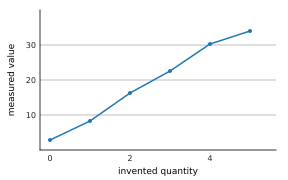
\includegraphics[width=0.8\textwidth]{figures/chart.svg}
\end{center}

A moving figure, described:

\begin{center}

\includegraphics[width=0.5\textwidth, alt={A pulsing invented signal}]{figures/pulse.svg}
\end{center}

Captions in translucent and reused groups, and shaded squares:

\begin{center}

\includegraphics[width=0.6\textwidth]{figures/captions.svg}

\includegraphics[width=0.3\textwidth]{figures/shades.svg}
\end{center}

A field of values drawn as an embedded raster:

\begin{center}
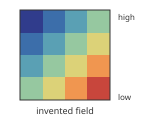
\includegraphics[width=0.5\textwidth]{figures/tiles.svg}
\end{center}
\end{document}
